\documentclass[a4paper,10pt]{amsart}
\usepackage{amssymb}
\usepackage[utf8]{inputenc}
\usepackage{tikz, fp, tikz-cd}
\usepackage[a4paper]{geometry}
\usepackage{mathtools}
\usepackage{multicol}
\usepackage{array}
\usepackage{stmaryrd}
\usepackage{csquotes}
\usepackage{environ} %package pour les macros d'édition
%\usepackage{subfigure}
\usepackage{subcaption}
\usepackage{shuffle}
\usepackage[english]{babel}
\usepackage{hyperref}

\usetikzlibrary{arrows}

%opening
\title{Efficient implementation of tridendriform Schroeder tree algebra}
\author{P. Catoire, L. Foissy, J. Fromentin}

\DeclareMathOperator{\Leaf}{Leaf}
\DeclareMathOperator{\lf}{lf}
\DeclareMathOperator{\Prim}{Prim}
\DeclareMathOperator{\ima}{Im}
\DeclareMathOperator{\Vect}{Vect}
\DeclareMathOperator{\car}{car}
\DeclareMathOperator{\Id}{Id}
\DeclareMathOperator{\IC}{InitChain}
\DeclareMathOperator{\internodes}{in}
\DeclareMathOperator{\Coass}{Coass}
\DeclareMathOperator{\Codend}{Codend}
\DeclareMathOperator{\Par}{Par}
\DeclareMathOperator{\Part}{\mathcal{P}}
\DeclareMathOperator{\Map}{Map}
\DeclareMathOperator{\bat}{Sh}
\DeclareMathOperator{\batc}{QSh}
\DeclareMathOperator{\Br}{Br}
\DeclareMathOperator{\K}{\mathbb{K}}

\newcommand\Sch{\mathsf{Sch}}
\newcommand\SchF{\mathsf{FSch}}
\newcommand\Schl{\mathsf{Sch}_\ell}
\newcommand\nn{n}
\newcommand\NN{\mathbb{N}}
\newcommand\pleft{\prec}
\newcommand\pmid{\cdot}
\newcommand\pright{\succ}
\newcommand{\IE}[2]{$\llbracket #1,#2 \rrbracket$}
\newcommand{\IEM}[2]{\llbracket #1,#2 \rrbracket}
\newcommand{\ssi}{if and only if}
\newcommand{\Schw}{Schroeder} %le mot Schroeder pour éviter les fautes de frappes


\newtheorem{thm}{Theorem}
\newtheorem{prop}{Proposition}
\theoremstyle{definition}
\newtheorem{exam}{Example}
\newtheorem{defi}{Definition}
\newtheorem{Not}{Notation}
\newtheorem{Rq}{Remark}

%%%%%%%%%%%%%%%%%%%%%%%%%%%%%%%%%%%%%%%%%%%%%%%%%%%%%%%%%%%
%%%%%%%%%%%%%%%%%%%%%%% Macros arbres %%%%%%%%%%%%%%%%%%%%%
%%%%%%%%%%%%%%%%%%%%%%%%%%%%%%%%%%%%%%%%%%%%%%%%%%%%%%%%%%

\newcommand{\Y}{\raisebox{-0.25\height}{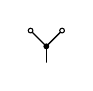
\begin{tikzpicture}[line cap=round,line join=round,>=triangle 45,x=0.2cm,y=0.2cm]
			\draw [line width=.5pt] (0.,0.)-- (0.,1.);
			\draw [line width=.5pt] (0.,1.)-- (-1.,2.);
			\draw [line width=.5pt] (0.,1.)-- (1.,2.);
			%marquages sommets
			\filldraw (0,1) circle(0.15);
			\draw[color=black, fill=white] (-1,2) circle (0.15);
			\draw[color=black, fill=white] (1,2) circle (0.15);
\end{tikzpicture}}}

\newcommand{\YY}{\raisebox{-0.3\height}{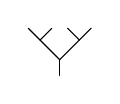
\begin{tikzpicture}[line cap=round,line join=round,>=triangle 45,x=0.2cm,y=0.2cm]
			\draw (0,0)--(0,1);
			\draw (0,1)--(-2,3);
			\draw (-1.25,2.25)--(-0.5,3);
			\draw (1.25,2.25)--(0.5,3);
			\draw (0,1)--(2,3);
\end{tikzpicture}}}

\newcommand{\peignedroit}[3]{\raisebox{-0.5\height}{\begin{tikzpicture}[line cap=round,line join=round,>=triangle 45,x=0.25cm,y=0.25cm]
			% Etage 1
			\draw (0,0)--(0,1);
			%Etage 2
			\draw (0,1)--(-1,2) node[left]{${#1}$};
			% Etage 3
			\draw (0,1)--(6,7);
			\draw (2,3)--(1,4) node[left]{${#2}$};
			%Etage...
			\draw (3.,4.5) node[rotate=45]{$\cdots$};
			%Etage k
			\draw (5,6)--(4,7) node[left]{${#3}$};
			%marquage des sommets
			\filldraw (0,1) circle (0.15);
			\filldraw (2,3) circle (0.15);
			\filldraw (5,6) circle (0.15);
			\draw[color=black, fill=white](6,7) circle (0.15);
\end{tikzpicture} }}

\newcommand{\peignegauche}[3]{\raisebox{-0.5\height}{\begin{tikzpicture}[line cap=round,line join=round,>=triangle 45,x=0.25cm,y=0.25cm]
			% Etage 1
			\draw (0,0)--(0,1);
			%Etage 2
			\draw (0,1)--(1,2) node[right]{${#1}$};
			% Etage 3
			\draw (0,1)--(-6,7);
			\draw (-2,3)--(-1,4) node[right]{${#2}$};
			%Etage...
			\draw (-3.,4.5) node[rotate=135]{$\cdots$};
			%Etage k
			\draw (-5,6)--(-4,7) node[right]{${#3}$};
			%marquage des sommets
			\filldraw (0,1) circle (0.15);
			\filldraw (-2,3) circle (0.15);
			\filldraw (-5,6) circle (0.15);
			\draw[color=black, fill=white](-6,7) circle (0.15);
\end{tikzpicture}}}

\newcommand{\balais}{\raisebox{-0.3\height}{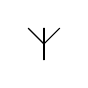
\begin{tikzpicture}[line cap=round,line join=round,>=triangle 45,x=0.2cm,y=0.2cm]
			\draw (0,0)--(0,2);
			\draw (0,1)-- (-1,2);
			\draw (0,1)-- (1,2);
\end{tikzpicture}}}
\newcommand{\balaisg}{\raisebox{-0.3\height}{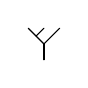
\begin{tikzpicture}[line cap=round,line join=round,>=triangle 45,x=0.2cm,y=0.2cm]
			\draw (0,0)-- (0,1);
			\draw (0,1)-- (-1,2);
			\draw (-0.5,1.5)-- (0,2);
			\draw (0,1)-- (1,2);
\end{tikzpicture}}}
\newcommand{\balaisd}{\raisebox{-0.3\height}{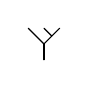
\begin{tikzpicture}[line cap=round,line join=round,>=triangle 45,x=0.2cm,y=0.2cm]
			\draw (0,0)-- (0,1);
			\draw (0,1)-- (-1,2);
			\draw (0.5,1.5)-- (0,2);
			\draw (0,1)-- (1,2);
\end{tikzpicture}}}
\DeclareDocumentCommand{\corollagraft}{m m m m}{\raisebox{-0.5\height}{\begin{tikzpicture}[line cap=round,line join=round,>=triangle 45,x=0.4cm,y=0.4cm]
			\draw (0,0)--(0,1);
			\draw (0,1)-- (-2,3) node[above,left] {$t_{#1}$};
			\draw (0,1)-- (-1,3) node[above] {$t_{#2}$};
			\draw (0,1)-- (1,3) node[above] {$t_{#3}$};
			\draw (0,1)-- (2,3) node[above,right] {$t_{#4}$};
			\draw (0,2.5) node[above] {$\dots$};
\end{tikzpicture}}}


%%%%%%%%%%%%%%%%%%%%%%%%%%%%%%%%%%%%%%%%%%%%%%%%%%%%%%%%%%%%%%%%%%%%%%%%%%%%%%%%%%%%%%%%%%%%%%%%%%%%%%%%%
%%%%%%%%%%%%%%%%%%%%% Macros d'édition pour laisser des commentaires %%%%%%%%%%%%%%%%%%%%%%%%%%%%%%%%%%%%%
%%%%%%%%%%%%%%%%%%%%%%%%%%%% ou montrer les changements %%%%%%%%%%%%%%%%%%%%%%%%%%%%%%%%%%%%%%%%%%%%%%%%%%
%%%%%%%%%%%%%%%%%%%%%%%%%%%%%%%%%%%%%%%%%%%%%%%%%%%%%%%%%%%%%%%%%%%%%%%%%%%%%%%%%%%%%%%%%%%%%%%%%%%%%%%%%%

%Pour les modifications

\NewEnviron{Jean}{{\color{red} \BODY }}
\NewEnviron{Pierre}{{\color{blue} \BODY }}
\NewEnviron{Loic}{{\color{olive} \BODY }}

% Macro faite pour supporter les sauts de lignes dans l'argument.

\newcommand{\JF}[1]{\begin{Jean}
		#1
\end{Jean}}
\newcommand{\PC}[1]{\begin{Pierre}
		#1
	\end{Pierre}{}}
\newcommand{\LF}[1]{\begin{Loic}
		#1
\end{Loic}}

%Pour les questions et remarque sur l'édition
% Attention, ne supporte pas les sauts de lignes dans l'argument.

\newcommand{\PCt}[1]{{\color{blue} \texttt{#1}}}
\newcommand{\JFt}[1]{{\color{red} \texttt{#1}}}
\newcommand{\LFt}[1]{{\color{olive} \texttt{#1}}}

\begin{document}

\maketitle

\section{Introduction}

\subsection{About the paper}


\subsection{Notations used in the article}

In this list, we put all a table of contents of notations used here :
\begin{itemize}
	\item $(\Sch, \pleft, \pmid, \pright)$ the graded tridendriform algebra on Schroeder tree;
	\item $\Sch(\nn)$ the set of Schroeder tree with $\nn$ leaves;
	\item $\SchF$ the set of forest of Schroeder tree.
\end{itemize}

\section{About the original problem}

\subsection{\Schw{} trees and comb representations}

Let us remind the following definition:
\begin{defi}
	A \emph{\Schw{} tree} is a rooted tree such that any vertices which is not a leaf has at least $2$ children.
	This set can be graded with the number of leaves minus $1$. For any $n\in\NN\setminus\{0\}$, we define $\Sch(\nn)$ the set of \Schw{} trees with $n+1$ leaves.
	We also put:
	\[
	\Sch\coloneqq \bigcup_{n=0}^{+\infty} \Sch(\nn).
	\]
\end{defi}
\begin{exam}\label{exam:Sch4}
	The elements of $\Sch(4)$ are
	\vspace{0.5em}
	\begin{center}
		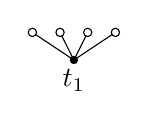
\begin{tikzpicture}[x=1em,y=1em]
			\draw(-1.5,1) -- (0,0);
			\draw(-0.5,1) -- (0,0);
			\draw(0.5,1) -- (0,0);
			\draw(1.5,1) -- (0,0);
			\draw[color=black, fill=white](-1.5,1) circle(0.15);
			\draw[color=black, fill=white](-0.5,1) circle(0.15);
			\draw[color=black, fill=white](0.5,1) circle(0.15);
			\draw[color=black, fill=white](1.5,1) circle(0.15);
			\fill(0,0) circle(0.15) node[below]{$t_1$};
		\end{tikzpicture}
		\hspace{1em}
		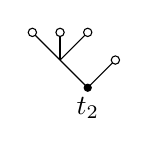
\begin{tikzpicture}[x=1em,y=1em]
			\draw(-1,2) -- (0,1);
			\draw(0,2) -- (0,1);
			\draw(1,2) -- (0,1);
			\draw(2,1) -- (1,0);
			\draw(0,1) -- (1,0);
			\draw[color=black, fill=white](-1,2) circle(0.15);
			\draw[color=black, fill=white](0,2) circle(0.15);
			\draw[color=black, fill=white](1,2) circle(0.15);
			\draw[color=black, fill=white](2,1) circle(0.15);
			\fill(1,0) circle(0.15) node[below]{$t_2$};
		\end{tikzpicture}
		\hspace{1em}
		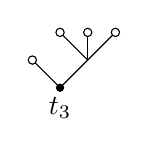
\begin{tikzpicture}[x=1em,y=1em]
			\draw(-1,1) -- (0,0);
			\draw(0,2) -- (1,1);
			\draw(1,2) -- (1,1);
			\draw(2,2) -- (1,1);
			\draw(1,1) -- (0,0);
			\draw[color=black, fill=white](-1,1) circle(0.15);
			\draw[color=black, fill=white](0,2) circle(0.15);
			\draw[color=black, fill=white](1,2) circle(0.15);
			\draw[color=black, fill=white](2,2) circle(0.15);
			\fill(0,0) circle(0.15) node[below]{$t_3$};
		\end{tikzpicture}
		\hspace{1em}
		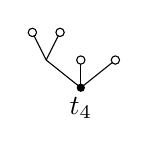
\begin{tikzpicture}[x=1em,y=1em]
			\draw(1,1) -- (-0.25,0);
			\draw(-0.25,1) -- (-0.25,0);
			\draw(-1,2) -- (-1.5,1);
			\draw(-2,2) -- (-1.5,1);
			\draw(-1.5,1) -- (-0.25,0);
			\draw[color=black, fill=white](1,1) circle(0.15);
			\draw[color=black, fill=white](-0.25,1) circle(0.15);
			\draw[color=black, fill=white](-1,2) circle(0.15);
			\draw[color=black, fill=white](-2,2) circle(0.15);
			\fill(-0.25,0) circle(0.15) node[below]{$t_4$};
		\end{tikzpicture}
		\hspace{1em}
		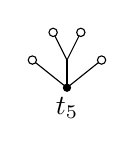
\begin{tikzpicture}[x=1em,y=1em]
			\draw(-0.25,2) -- (0.25,1);
			\draw(0.75,2) -- (0.25,1);
			\draw(-1,1) -- (0.25,0);
			\draw(0.25,1) -- (0.25,0);
			\draw(1.5,1) -- (0.25,0);
			\draw[color=black, fill=white](-1,1) circle(0.15);
			\draw[color=black, fill=white](-0.25,2) circle(0.15);
			\draw[color=black, fill=white](0.75,2) circle(0.15);
			\draw[color=black, fill=white](1.5,1) circle(0.15);
			\fill(0.25,0) circle(0.15) node[below]{$t_5$};
		\end{tikzpicture}
		\hspace{1em}
		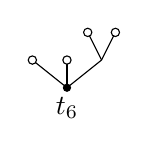
\begin{tikzpicture}[x=1em,y=1em]
			\draw(-1,1) -- (0.25,0);
			\draw(0.25,1) -- (0.25,0);
			\draw(1,2) -- (1.5,1);
			\draw(2,2) -- (1.5,1);
			\draw(1.5,1) -- (0.25,0);
			\draw[color=black, fill=white](-1,1) circle(0.15);
			\draw[color=black, fill=white](0.25,1) circle(0.15);
			\draw[color=black, fill=white](1,2) circle(0.15);
			\draw[color=black, fill=white](2,2) circle(0.15);
			\fill(0.25,0) circle(0.15) node[below]{$t_6$};
		\end{tikzpicture}
		\vspace{1em}
	\end{center}
	\begin{center}
		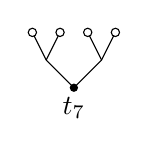
\begin{tikzpicture}[x=1em,y=1em]
			\draw(0,2) -- (0.5,1);
			\draw(1,2) -- (0.5,1);
			\draw(2,2) -- (2.5,1);
			\draw(3,2) -- (2.5,1);
			\draw(0.5,1) -- (1.5,0);
			\draw(2.5,1) -- (1.5,0);
			\draw[color=black, fill=white](0,2) circle(0.15);
			\draw[color=black, fill=white](1,2) circle(0.15);
			\draw[color=black, fill=white](2,2) circle(0.15);
			\draw[color=black, fill=white](3,2) circle(0.15);
			\fill(1.5,0) circle(0.15) node[below]{$t_7$};
		\end{tikzpicture}
		\hspace{1em}
		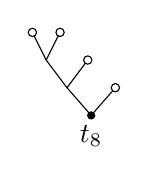
\begin{tikzpicture}[x=1em,y=1em]
			\draw(-1,2) -- (-0.5,1);
			\draw(0,2) -- (-0.5,1);
			\draw(1,1) -- (0.25,0);
			\draw(-0.5,1) -- (0.25,0);
			\draw(0.25,0) -- (1.125, -1);
			\draw(2,0) -- (1.125, -1);
			\draw[color=black, fill=white](-1,2) circle(0.15);
			\draw[color=black, fill=white](0,2) circle(0.15);
			\draw[color=black, fill=white](1,1) circle(0.15);
			\draw[color=black, fill=white](2,0) circle(0.15);
			\fill(1.125,-1) circle(0.15) node[below]{$t_8$};
		\end{tikzpicture}
		\hspace{1em}
		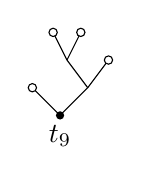
\begin{tikzpicture}[x=1em,y=1em]
			\draw(-1,2) -- (-0.5,1);
			\draw(0,2) -- (-0.5,1);
			\draw(1,1) -- (0.25,0);
			\draw(-0.5,1) -- (0.25,0);
			\draw(0.25,0) -- (-0.75,-1);
			\draw(-1.75,0) -- (-0.75,-1);
			\draw[color=black, fill=white](-1,2) circle(0.15);
			\draw[color=black, fill=white](0,2) circle(0.15);
			\draw[color=black, fill=white](1,1) circle(0.15);
			\draw[color=black, fill=white](-1.75,0) circle(0.15);
			\fill(-0.75,-1) circle(0.15) node[below]{$t_9$};
		\end{tikzpicture}
		\hspace{1em}
		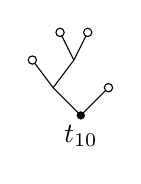
\begin{tikzpicture}[x=1em,y=1em]
			\draw(1,2) -- (0.5,1);
			\draw(0,2) -- (0.5,1);
			\draw(-1,1) -- (-0.25,0);
			\draw(0.5,1) -- (-0.25,0);
			\draw(-0.25,0) -- (0.75,-1);
			\draw(1.75,0) -- (0.75,-1);
			\draw[color=black, fill=white](1,2) circle(0.15);
			\draw[color=black, fill=white](0,2) circle(0.15);
			\draw[color=black, fill=white](-1,1) circle(0.15);
			\draw[color=black, fill=white](1.75,0) circle(0.15);
			\fill(0.75,-1) circle(0.15) node[below]{$t_{10}$};
		\end{tikzpicture}
		\hspace{1em}
		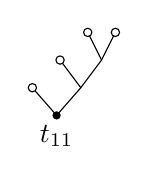
\begin{tikzpicture}[x=1em,y=1em]
			\draw(1,2) -- (0.5,1);
			\draw(0,2) -- (0.5,1);
			\draw(-1,1) -- (-0.25,0);
			\draw(0.5,1) -- (-0.25,0);
			\draw(-0.25,0) -- (-1.125, -1);
			\draw(-2,0) -- (-1.125, -1);
			\draw[color=black, fill=white](1,2) circle(0.15);
			\draw[color=black, fill=white](0,2) circle(0.15);
			\draw[color=black, fill=white](-1,1) circle(0.15);
			\draw[color=black, fill=white](-2,0) circle(0.15);
			\fill(-1.125,-1) circle(0.15) node[below]{$t_{11}$};
		\end{tikzpicture}
	\end{center}
\end{exam}


\begin{Rq}
	As every node of these trees which is not a leaf has at least $2$ children, we will not draw the nodes of a tree any more.
\end{Rq}

Let $t$ be a tree. It $t$ can always be seen as:
\begin{center}
	\raisebox{-0.5\height}{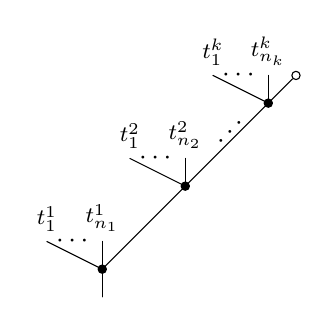
\begin{tikzpicture}[line cap=round,line join=round,x=1em,y=1 em]
			% Etage 1
			\draw (0,0)--(0,1);
			\filldraw (0,1) circle (0.15);
			%Etage 2
			\draw (0,1)--(-2,2)
			 node[above]{\footnotesize{$t^1_1$}};
			\draw (0,1)--(0,2) node[above]{\footnotesize{$t^1_{n_1}$}};
			\draw (-1,2) node{$\cdots$};
			% Etage 3
			\draw (0,1)--(7,8);
			\filldraw[color=white] (7,8) circle (0.15);
			\draw (3,4)--(1,5) node[above]{\footnotesize{$t^2_1$}};
			\filldraw (3,4) circle (0.15);
			\draw (3,4)--(3,5) node[above]{\footnotesize{$t^2_{n_2}$}};
			\draw (2,5) node{$\cdots$};
			%Etage...
			\draw (4.7,6) node[rotate=45]{$\cdots$};
			%Etage k
			\draw[color=black, fill=white](7,8) circle(0.15);
			\filldraw (6,7) circle (0.15);
			\draw (6,7)--(4,8) node[above]{\footnotesize{$t^k_1$}};
			\draw (6,7)--(6,8) node[above]{\footnotesize{$t^k_{n_k}$}};
			\draw (5,8) node {$\cdots$};
	\end{tikzpicture}},
\end{center}
where $k$ is the number of nodes on the right-most branch of $t$ and for $i\in\IEM{1}{k}, n_i+1$ is the number of sons of the $i$-th node of this branch.

\begin{Not}
	Let $F=t_1\dots t_n$ be a forest composed of $n$ trees. Instead of writing:
	\begin{center}
		\raisebox{-0.5\height}{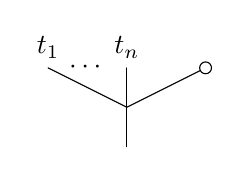
\begin{tikzpicture}[line cap=round,line join=round,x=0.5cm,y=0.5cm]
				% Etage 1
				\draw (0,0)--(0,1);
				%Etage 2
				\draw (0,1)--(-2,2) node[left,above]{$t_1$};
				\draw (0,1)--(0,2) node[right,above]{$t_{n}$};
				\draw (-1,2) node{$\cdots$};
				\draw (0,1)--(2,2);
				\draw[color=black, fill=white] (2,2) circle (0.15);
		\end{tikzpicture}},
	\end{center}
	we will write:
	\raisebox{-0.3\height}{\begin{tikzpicture}[line cap=round,line join=round,x=0.3cm,y=0.3cm]
			% Etage 1
			\draw (0,0)--(0,1);
			%Etage 2
			\draw (0,1)--(-1,2) node[left]{$F$};
			\draw (0,1)--(1,2);
			\draw[color=black, fill=white] (1,2) circle (0.15);
	\end{tikzpicture}}.
\end{Not}

With these notations, we notice that all tree $t$ can be seen either  respectively like a \emph{right comb} or a \emph{left comb}:
\begin{align*}
	t&=\peignedroit{F_1}{F_2}{F_k}
	& \text{ and } &&  s=\peignegauche{F_{k+1}}{F_{k+2}}{F_{k+l}},
\end{align*}
where $F_1,\dots,F_k$ and $F_{k+1},\dots, F_{k+l}$ are non-empty forests.
\begin{defi}
	The writing defined above is the writing of $t$ as a \emph{right comb}.
	Proceeding the same way, looking at the left branch of the root of $t$, we get the writing of $t$ as a \emph{left comb}.
\end{defi}


\subsection{Our objective}

\begin{defi}\label{def:tridend}
	Let $\K$ be a field and $A$ be vector space of $\K$. We say $(A,\prec,\cdot,\succ)$ is a \emph{tridendriform algebra} if $\prec,\cdot$ and $\succ$ are all linear maps from $A\otimes A$ to $A$ such that for any $a,b,c\in A$:
	\begin{align}
		(a\prec b)\prec c&=a\prec(b*c), \label{eq:tri1}\\
		(a\succ b)\prec c&=a\succ(b\prec c), \label{eq:tri2} \\
		(a* b)\succ c&=a\succ(b\succ c),  \label{eq:tri3} \\
		(a\succ b)\cdot c&=a\succ(b\cdot c), \label{eq:tri4} \\
		(a\prec b)\cdot c&=a\cdot(b\succ c), \label{eq:tri5} \\
		(a\cdot b)\prec c&=a\cdot(b\prec c), \label{eq:tri6} \\
		(a\cdot b)\cdot c&=a\cdot (b\cdot c), \label{eq:tri7}
	\end{align}
	where $*$ is the \emph{associative product} of the tridendriform algebra defined for any $a,b\in A$ by $a*b\coloneqq a\prec b + a\cdot b +a\succ b$. 
	We call the products $\succ,\prec,\cdot$ respectively right, left and middle.
\end{defi} 

The free tridendriform algebra is built on the vector space $\K\Sch \oplus \K\cdot |$ where $|$ is the unit of the product $*$. We will denote it by $(\Sch{},\prec,\cdot,\succ)$. We have a combinatorial interpretation of the product $*$. For this let us introduce:
\begin{defi}[Quasi-shuffle]
	Let $k,l\in\NN\setminus \{0\}$. A \emph{$(k,l)$-quasi-shuffle} is a surjective map $\sigma:\IEM{1}{k+l}\twoheadrightarrow\IEM{1}{n}$ surjective for some positive integer $n$
	such that:
	\[
	\sigma(1)<\cdots<\sigma(k) \text{  and  } \sigma(k+1)<\cdots<\sigma(k+l).
	\]
	We will denote $\batc(k,l)$ the set of all $(k,l)$-quasi-shuffles.
\end{defi}


Let $t,s$ two trees different from $|$. We look $t$ as a right comb and $s$ as a left comb. In other words, we put:
\begin{align*}
	t&=\peignedroit{F_1}{F_2}{F_k}
	& \text{ and } &&  s=\peignegauche{F_{k+1}}{F_{k+2}}{F_{k+l}},
\end{align*}
where for all $i\in\IEM{1}{k+l}, F_i$ is a non-empty forest. Here, $k$ represents the number of nodes on the right-most branch of $t$ and $l$ is the number of nodes on the left-most branch of $s$.

\begin{defi}\label{def:quasiaction}
	Let $t$ and $s$ be two trees which respective right comb representation and left comb representation are given above.
	We denote by $k$ (respectively $l$) the number of nodes on the right-most (respectively left-most) branch of $t$ (respectively $s$). Let $\sigma$ be a $(k,l)$-quasi-shuffle which has for image $\IEM{1}{n}$ for $n$ a positive integer. We denote $\sigma(t,s)$ the tree obtained this way:
	\begin{enumerate}
		\item  We first consider the ladder with $n$ nodes:
		\begin{center}
			\raisebox{-0.5\height}{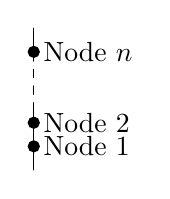
\begin{tikzpicture}[line cap=round,line join=round,>=triangle 45,x=0.3cm,y=0.3cm]
					\begin{scope}{shift={(-3,0)}}
						\draw (0,0)--(0,2.5);
						\draw[dashed] (0,2.5)--(0,5);
						\draw (0,5)--(0,6);
						\filldraw [black] (0,1) circle (2pt) node[anchor=west]{Node $1$};
						\filldraw [black] (0,2) circle (2pt) node[anchor=west]{Node $2$};
						\filldraw [black] (0,5) circle (2pt) node[anchor=west]{Node $n$};
					\end{scope}
			\end{tikzpicture}}.
		\end{center}
		\item For all $i\in\IEM{1}{k},$ we graft $F_i$ as the \emph{left} son at the node $\sigma(i)$.
		\item For all $i\in\IEM{k+1}{k+l},$ we graft $F_i$ as \emph{right} son at the node $\sigma(i)$.
	\end{enumerate}
\end{defi}

\begin{exam}\label{exam:quasiaction}
	Consider the $(2,2)$-quasi-shuffle $\sigma=(1,3,2,3)$. Let us take 
	$t=$	\raisebox{-0.3\height}{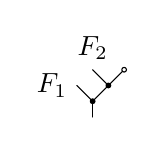
\begin{tikzpicture}[line cap=round,line join=round,>=triangle 45,x=0.2cm,y=0.2cm]
			% Etage 1
			\draw (0,0)--(0,1);
			%Etage 2
			\draw (0,1)--(-1,2) node[left]{$F_1$};
			% Etage 3
			\draw (0,1)--(2,3);
			\draw (1,2)--(0,3) node[left,above]{$F_2$};
			%marquages des sommets
			\filldraw (0,1) circle (0.15);
			\filldraw (1,2) circle (0.15);
			\draw[color=black, fill=white] (2,3) circle (0.15);
	\end{tikzpicture}} and $s=\raisebox{-0.3\height}{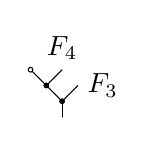
\begin{tikzpicture}[line cap=round,line join=round,>=triangle 45,x=0.2cm,y=0.2cm]
			% Etage 1
			\draw (0,0)--(0,1);
			%Etage 2
			\draw (0,1)--(1,2) node[right]{$F_{3}$};
			% Etage 3
			\draw (0,1)--(-2,3);
			\draw (-1,2)--(0,3) node[right,above]{$F_{4}$};
			%marquages des sommets
			\filldraw (0,1) circle (0.15);
			\filldraw (-1,2) circle (0.15);
			\draw[color=black, fill=white] (-2,3) circle (0.15);
	\end{tikzpicture}}$.
	Then $\sigma(t,s)=$\raisebox{-0.5\height}{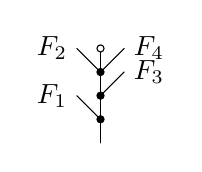
\begin{tikzpicture}[line cap=round,line join=round,>=triangle 45,x=0.3cm,y=0.3cm]
			\draw (0,0)--(0,4);
			%Noeud 1
			\draw (0,1)--(-1,2) node[left]{$F_1$};
			%Noeud 2
			\draw (0,2)--(1,3) node[right]{$F_3$};
			%Noeud 3
			\draw (0,3)--(-1,4) node[left]{$F_2$};
			\draw (0,3)--(1,4) node[right]{$F_4$};
			%marquage des noeuds
			\filldraw (0,1) circle (0.15);
			\filldraw (0,2) circle (0.15);
			\filldraw (0,3) circle (0.15);
			\draw[color=black, fill=white] (0,4) circle (0.15);
	\end{tikzpicture}}.
\end{exam} 

\begin{thm}\label{thm:produit}
	Let $t,s$ be two trees different from $|$ as described above. Then: 
	\[
	t*s=\sum_{\sigma\in \batc(k,l)}\sigma(t,s).
	\]
	Moreover:
	\begin{gather*}
		t\prec s=\sum_{\substack{\sigma\in\batc(k,l) \\ \sigma^{-1}(\{1\})=\{1\}}} \sigma(t,s), 
		 t\succ s=\sum_{\substack{\sigma\in\batc(k,l) \\ \sigma^{-1}(\{1\})=\{k+1\}}} \sigma(t,s),\\
		t\cdot s=\sum_{\substack{\sigma\in\batc(k,l) \\ \sigma^{-1}(\{1\})=\{1,k+1\}}} \sigma(t,s).
	\end{gather*}
\end{thm}
Surprisingly,  $(\Sch,\prec,\cdot,\succ)$ can be endowed with a codendriform coproduct:
\begin{thm}\label{thm:coproduit}
	We define a map $\Delta:\K\Sch\rightarrow \K\Sch\otimes \K\Sch$ by:
	\begin{align*}
		\Delta(t)=\sum_{c \text{ \normalfont admissible cut of }t} P^c(t)\otimes R^c(t),
	\end{align*}
	where $R^c(t)$ is the component of $t$ containing its root and $P^c(t)=P^c_1(t)*\cdots *P^c_k(t)$, where $P^c_i(t)$ are the cut trees naturally ordered from left to right. Moreover one can write $\Delta=\Delta_{\leftarrow}+\Delta_{\rightarrow}$ in such a way so $(\Sch,\prec,\cdot,\succ,\Delta_{\leftarrow},\Delta_{\rightarrow})$ is a $(3,2)$-dendriform bialgebra detailled in~\cite{2023_Cat}.
\end{thm}

From the Cartier-Quillen-Milnor-Moore theorem, we can understand better the cocommutative part of this Hopf algebra from its primitives.
Hence, a natural question is to compute the primitives of $\Sch$. Let us introduce the notations to reach the theorems for this purpose:
\begin{defi}
	Let $(C,\Delta_{\leftarrow},\Delta_{\rightarrow})$ be a dendriform coalgebra. We define:
	\begin{gather*}
		\Prim_{\leftarrow}(C):=\{ c\in C \,|\, \tilde{\Delta}_{\leftarrow}(c)=0 \}, 
		\Prim_{\rightarrow}(C):=\{ c\in C \,|\, \tilde{\Delta}_{\rightarrow}(c)=0 \}, \\
		\Prim_{\Coass}(C):=\{ c\in C \,|\, \tilde{\Delta}(c)=0 \},
		\Prim_{\Codend}(C):=\{ c\in C \,|\, \tilde{\Delta}_{\leftarrow}(c)=\tilde{\Delta}_{\rightarrow}(c)=0 \}.
	\end{gather*}
\end{defi}

\begin{thm}\label{thm:coassincodend}
	For all $n\in\NN$, we define:
	\begin{equation*}
		\theta_n:\left\lbrace \begin{array}{rcl}
			\Prim_{\Coass}(\Sch(n))& \rightarrow & \Prim_{\Codend}(\Sch(n+1)), \\
			a\otimes \Y & \mapsto & a\cdot \Y.
		\end{array}\right.
	\end{equation*}
	Then, for all $n\in\NN, \theta_n$ is an isomorphism of vector spaces.
\end{thm}

From the article~\cite{euleridem} of M.Ronco, we recall the main result:
\begin{thm}\label{thm:génération2}
	 One can define  a map $\omega$ using $\pright,\pmid$ and $\pleft$ giving rise for all $n\in\NN$ to:
	\begin{equation}\label{eq:Omega}
		\Omega_n:\left\lbrace\begin{array}{rcl}
			T(\Prim_{\Codend}(\Sch(n))) & \twoheadrightarrow & \Prim_{\Coass}(\Sch(n)), \\
			x_1\otimes\dots\otimes x_k & \mapsto & \omega(x_1\otimes \dots \otimes x_k).
		\end{array}\right.
	\end{equation}
	This raise to a map $\Omega$ defined over $\Sch$ such that $\Omega|_{T(\Prim_{\Codend}(\Sch(n)))}=\Omega_n$.
\end{thm}

As a consequence, we have a recipe to produce the primitives of this algebra by induction as shown in figure~\cite{fig:algo_idea}:
\begin{figure}[h]
	\centering
	\begin{tikzcd}
		\Prim_{\Codend}(\Sch(1)) \arrow[r,"\theta_1"] &\Prim_{\Coass}(\Sch(2)) \arrow[r,"\Omega_1"] & \Prim_{\Codend}(\Sch(2)) \arrow[r,"\theta_1"] & \Prim_{\Codend}(\Sch(3)) \arrow[r,"\Omega_2"]& \dots
	\end{tikzcd}
	\caption{Diagram of the induction}
	\label{fig:algo_idea}
\end{figure}

This figure~\ref{fig:algo_idea} enables us to compute $\Prim_{\Coass}(\Sch)$ by induction over the degree of its elements starting with $\Prim_{\Codend}(\Sch(1))=\left\{\Y\right\}$. We will now look at the practical aspects to implement an algorithm on a computer. 

\section{Our point of view of Schroeder trees and their operations}

Our motivation is to compute the process detailed in figure~\ref{fig:algo_idea}. First to describe some primitives elements and second to try and guess an explicit combinatorial formula describing this process.
But a question arise from this: \textquote{How shall we implement trees to get efficiency and a easy code ?} 

\subsection{Encoding \Schw{} trees}

The idea to represent \Schw{} trees into a computer is to add \emph{levels} giving rise to \emph{levelled \Schw{} trees}. From this intermediate representation, we can interpret a \Schw{} tree as a sequence of integers whose binary code represents the levels of the tree.

\subsubsection{Levelled Schroeder Tree}

\begin{defi}
	%définition des heap-order et arbres de Sch à niveaux à mettre ici
	The set of levelled \Schw{} tree is denoted $\Schl$ while the levelled \Schw{} trees with $n$ leaves is denoted $\Schl(\nn)$.
\end{defi}
To each levelled \Schw{} tree corresponds a unique Schroeder tree we have a trivial surjection
\begin{equation}
	\pi_\nn:\Schl(\nn)\twoheadrightarrow\Sch(\nn).
\end{equation}
Maps $\pi_0$, $\pi_1$, $\pi_2$ and $\pi_3$ are bijective while $\pi_\nn$ is not injective for $n\geq 4$.

\begin{defi}
	Two levelled tree $t$ and $t'$ of $\Schl(\nn)$ are said \emph{equivalent}, denoted $t\equiv t'$, if it represents the same Schroeder tree, that is, $\pi_\nn(t)=\pi_\nn(t')$.
\end{defi}

\begin{exam}\label{exam:Sch}
	Referring to the example~\ref{exam:Sch4}, except for $i=7$, the set $\pi_4^{-1}(t_i)$ has only one element.
For example $\pi_4^{-1}(t_8)$ consists of the unique levelled tree:
\begin{center}
	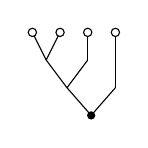
\begin{tikzpicture}[x=1em,y=1em]
		\draw(0,3) -- (0.5,2);
		\draw(1,3) -- (0.5,2);
		\draw(2,3) -- (2,2);
		\draw(3,3) -- (3,2) -- (3,1);
		\draw(0.5,2) -- (1.25,1);
		\draw(2,2) -- (1.25,1);
		\draw(1.25,1) -- (2.125, 0);
		\draw(3,1) -- (2.125, 0);
		\draw[color=black, fill=white](0,3) circle(0.15);
		\draw[color=black, fill=white](1,3) circle(0.15);
		\draw[color=black, fill=white](2,3) circle(0.15);
		\draw[color=black, fill=white](3,3) circle(0.15);
		\fill(2.125,0) circle(0.15);
	\end{tikzpicture}
\end{center}
Labelled trees in $\pi_4^{-1}(t_7)$ consists of the following two levelled trees:
\begin{center}
	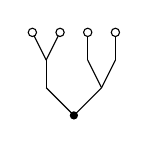
\begin{tikzpicture}[x=1em,y=1em]
		\draw(0,3) -- (0.5,2);
		\draw(1,3) -- (0.5,2);
		\draw(2,3) -- (2,2);
		\draw(3,3) -- (3,2);
		\draw(2,2) -- (2.5,1);
		\draw(3,2) -- (2.5,1);
		\draw(0.5,2) -- (0.5,1);
		\draw(0.5,1) -- (1.5,0);
		\draw(2.5,1) -- (1.5,0);
		\draw[color=black, fill=white](0,3) circle(0.15);
		\draw[color=black, fill=white](1,3) circle(0.15);
		\draw[color=black, fill=white](2,3) circle(0.15);
		\draw[color=black, fill=white](3,3) circle(0.15);
		\fill(1.5,0) circle(0.15);
	\end{tikzpicture}
	\hspace{2em}
	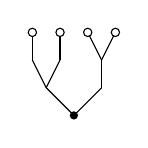
\begin{tikzpicture}[x=1em,y=1em]
		\draw(0,3) -- (0,2);
		\draw(1,3) -- (1,2);
		\draw(2,3) -- (2.5,2);
		\draw(3,3) -- (2.5,2);
		\draw(0,2) -- (0.5,1);
		\draw(1,2) -- (0.5,1);
		\draw(2.5,2) -- (2.5,1);
		\draw(0.5,1) -- (1.5,0);
		\draw(2.5,1) -- (1.5,0);
		\draw[color=black, fill=white](0,3) circle(0.15);
		\draw[color=black, fill=white](1,3) circle(0.15);
		\draw[color=black, fill=white](2,3) circle(0.15);
		\draw[color=black, fill=white](3,3) circle(0.15);
		\fill(1.5,0) circle(0.15);
	\end{tikzpicture}
\end{center}

\end{exam}
We want to code \Schw{} trees as levelled Schroeder trees. For this purpose, we need to make a choice of a representative levelled \Schw{} tree of each \Schw{} tree.  

\subsubsection{Our point of view on \Schw{} trees}
\begin{defi}[Initial chains]
	Let $\mathcal{P}=(P,\leq)$ be a lattice with a minimum and a maximum element.
	Let $C$ be a chain in this poset, we say it is \emph{initial} if $\min(\mathcal{P})$ and $\max(\mathcal{P})$ are in the chain $C$.
\end{defi}

\begin{defi}
	Let $n\in\NN\setminus \{0\}$.
	We define $\IC(\nn)$ the set of strictly increasing \emph{initial chain} of the poset $(\Par(\IEM{1}{n}),\leqslant_{\pi})$ where $\leqslant_\pi$ is the \emph{refinement order} of partitions. 
\end{defi}
\begin{exam}
	For instance, in the poset $(\Par(\IEM{1}{4}),\supseteq)$ shown in figure~\ref{fig:labelled_IP4}, we have the following elements of $\IC(4)$:
	\begin{gather*}
		\{1\}\{2\}\{3\}\{4\}\leqslant_{\pi} \{1,2,3,4\}, \\
		\{1\}\{2\}\{3\}\{4\}\leqslant_{\pi} \{1,2,3\}\{4\} \leqslant_{\pi} \{1,2,3,4\}.
	\end{gather*}
\end{exam}
\begin{figure}[h]
	\centering
	\caption{The $\mathcal{P}(\IEM{1}{4})$ poset with labels on edges}
	\label{fig:labelled_IP4}
	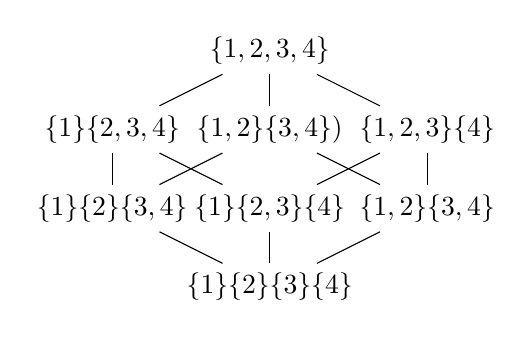
\begin{tikzpicture}[rotate =180 ]
		%Noeud du diagramme
		\node (P0) at (0,0) {$\{1,2,3,4\}$};
		\node (P11) at (-2,1) {$\{1,2,3\}\{4\}$};
		\node (P12) at (0,1) {$\{1,2\}\{3,4\})$};
		\node (P13) at (2,1) {$\{1\}\{2,3,4\}$};
		\node(P21) at (-2,2) {$\{1,2\}\{3,4\}$};
		\node(P22) at (0,2) {$\{1\}\{2,3\}\{4\}$};
		\node(P23) at (2,2) {$\{1\}\{2\}\{3,4\}$};
		\node(P31) at (0,3) {$\{1\}\{2\}\{3\}\{4\}$};
		%Arêtes du poset
		\draw (P0) -- (P11);
		\draw (P0) -- (P12);
		\draw (P0) -- (P13);
		\draw (P11) -- (P21);
		\draw (P11) -- (P22);
		\draw (P12) -- (P21);
		\draw (P12) -- (P23);
		\draw (P13) -- (P22);
		\draw (P13) -- (P23);
		\draw (P21) -- (P31);
		\draw (P22) -- (P31);
		\draw (P23) -- (P31);
	\end{tikzpicture}
\end{figure}

But as said previously many levelled \Schw{} trees give a same \Schw{} tree. Hence, for each $n\in \NN$ we want to construct a section of $\pi_n$ so that a \emph{unique} levelled \Schw{} tree corresponds to a \Schw{} tree.

\subsubsection{Our choice of section}

For our use, we introduce the following map:
\begin{prop}
	We denote $s:\Sch \rightarrow \Schl$ the unique map such that for any $t\in\Sch(n)$, $s(t)$ is the \emph{unique} levelled \Schw{} tree such that for any internal vertices $t$ its level is greater than all the internal vertices to its right.
	Then, $s$ is well-defined and this is a section to the map $\pi\coloneqq \displaystyle\bigoplus_{n=0}^{+\infty} \pi_n$.
\end{prop}
\begin{proof}
	To prove $s$ is well-defined, we detail a construction $s(t)$ by induction over the number of leaves of the tree of $t$. Let $t\in\Sch(n)$ with $n\in\NN^*$.
	\begin{description}
		\item[Initialization] for $n=2$, this is obvious as there exists only one representation of $\Y$ as a levelled \Schw{} tree.  
		\item[Heredity] now let us suppose that there exists $n$ such that for any $t\in\Sch(n), s(t)$ is well defined. We consider $t\in\Sch(n+1)$ and let us build $s(t)$. One can see:
		\[
		t=t^{(1)}\vee \dots \vee t^{(k)}
		\]
		where for any $k\geq 2, i\in\IEM{1}{k}, t^{(i)}$ is a \Schw{} tree with at most $n$ leaves.
		Hence, we built $s(t)$ as follows:
		\[
		s(t)=
			\peignegauche{s(t^{(1)})}{s(t^{(2)})}{s(t^{(k)})}
		\]
	\end{description}
	Finally by construction, we have $\pi\circ s=\Id_{\K\Sch}$ 	
\end{proof}
\begin{exam}
	Consider the tree
	\begin{center}
	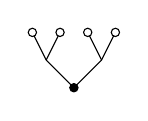
\begin{tikzpicture}[x=1em,y=1em]
		\draw(0,2) -- (0.5,1);
		\draw(1,2) -- (0.5,1);
		\draw(2,2) -- (2.5,1);
		\draw(3,2) -- (2.5,1);
		\draw(0.5,1) -- (1.5,0);
		\draw(2.5,1) -- (1.5,0);
		\draw[color=black, fill=white](0,2) circle(0.15);
		\draw[color=black, fill=white](1,2) circle(0.15);
		\draw[color=black, fill=white](2,2) circle(0.15);
		\draw[color=black, fill=white](3,2) circle(0.15);
		\filldraw[color=black] (1.5,0) circle(0.15);
	\end{tikzpicture}
\end{center}
	The only tree satisfying this definition among its two representatives is:
	\begin{center}
		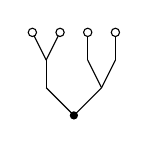
\begin{tikzpicture}[x=1em,y=1em]
			\draw(0,3) -- (0.5,2);
			\draw(1,3) -- (0.5,2);
			\draw(2,3) -- (2,2);
			\draw(3,3) -- (3,2);
			\draw(2,2) -- (2.5,1);
			\draw(3,2) -- (2.5,1);
			\draw(0.5,2) -- (0.5,1);
			\draw(0.5,1) -- (1.5,0);
			\draw(2.5,1) -- (1.5,0);
			\draw[color=black, fill=white](0,3) circle(0.15);
			\draw[color=black, fill=white](1,3) circle(0.15);
			\draw[color=black, fill=white](2,3) circle(0.15);
			\draw[color=black, fill=white](3,3) circle(0.15);
			\fill(1.5,0) circle(0.15);
		\end{tikzpicture}
	\end{center}
\end{exam}

For the sequel let us introduce some definitions

\begin{defi}
	Let $t$ be a tree. Let $v$ be a vertex in $t$. We say that $v$ is an \emph{internal vertex} if it is not a leaf.
	We will denote $\in(t)$ the number of internal vertices of $t$. Note that for \Schw{} trees this quantity is always non-negative.
\end{defi}

Using the section $s$, we can identify to any \Schw{} tree a finite list of binary words thanks to the map defined below

\begin{defi}
	For any $n\in\NN,$ we introduce a map $\varphi_n: \Schl(n)\rightarrow \IC(\IEM{1}{n})$ defined for any $t\in\Schl(n)$ by the \emph{unique} initial chain describing the life time of the angles of $t$ in function of the levels of the tree.
\end{defi}
\begin{exam}\label{Eg:tree_code}
	For instance:
	\begin{align}
		\raisebox{-0.5\height}{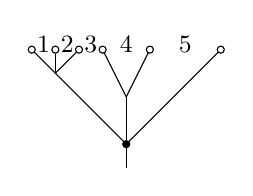
\begin{tikzpicture}[x=0.3cm, y=0.3cm]
				\draw (0,0)--(0,1);
				\draw (0,1)--(-4,5);
				\draw (0,1)--(4,5);
				\draw (0,1)--(0,3);
				\draw (0,3)--(-1,5);
				\draw (0,3)--(1,5);
				\draw (-3,4)--(-2,5);
				\draw (-3,4)--(-3,5);
				% dessin des noeuds
				\filldraw (0,1) circle (0.15);
				\draw[ color=black, fill=white]  (-4,5) circle (0.15);
				\draw[ color=black, fill=white]  (-3,5) circle (0.15);
				\draw[ color=black, fill=white]  (-2,5) circle (0.15);
				\draw[ color=black, fill=white]  (-1,5) circle (0.15);
				\draw[ color=black, fill=white]  (4,5) circle (0.15);
				\draw[ color=black, fill=white]  (1,5) circle (0.15);
				% Décorations angulaires
				\draw (-3.5, 5.2) node{\small{$1$}};
				\draw (-2.5, 5.2) node{\small{$2$}};
				\draw (-1.5,5.2) node{\small{$3$}};
				\draw (0, 5.2) node{\small{$4$}};
				\draw (2.5, 5.2) node{\small{$5$}};
		\end{tikzpicture}} && \rightarrow && \begin{array}{c}
			\IEM{1}{5} \\
			\IEM{3}{5} \\
			\{3\}~\{5\} \\
			\emptyset
		\end{array}
%		&& \rightarrow &&  \begin{array}{ccccc}
%			0 & 0 & 0 & 0 & 0 \\
%			1 & 1 & 0 & 0 & 0 \\
%			1 & 1 & 0 & 1 & 0 \\
%			1 & 1 & 1 & 1 & 1
%		\end{array} && \rightarrow && \begin{array}{c}
%			0 \\ 3 \\ 11 \\ 15
%		\end{array}
	\end{align}
\end{exam}

Thanks to this result we can now encode one \Schw{} tree as a list of integers into a computer. Now, we can look at the action of quasi-shuffles on our encoding of trees for an easy computation in the free tridendriform algebra with one generator.
 
%\subsubsection{The tridendriform structure for levelled \Schw{} trees}
%
%%\PCt{To be edited}

\section{Coding the problem}


\bibliographystyle{plain}
\bibliography{article.bib}

\end{document}
